\documentclass[a4paper,11pt,oneside]{book}
\usepackage[spanish]{babel}
\usepackage[utf8]{inputenc}
\usepackage[margin=1in]{geometry}
\usepackage{hyperref,xcolor,fancyhdr}
\usepackage{graphicx}
\graphicspath{ {Figuras/} }
\pagestyle{fancy}
\setlength{\parskip}{2mm}
\usepackage{tcolorbox}
\tcbuselibrary{listingsutf8}



\title{Práctica 1 - Introducción a APKs en Android}
\author{Jaime García González}
\date{}


\begin{document}
\maketitle
\tableofcontents


\chapter{Introducción}

\chapter{Desarrollo de una aplicación Android}

\chapter{Estudio de kontaktos.apk}


\section{Verificación de firma}

En este apartado se procederá a verificar la firma de la aplicación \emph{kontaktos.apk}, para ello, se utilizará la herramienta \emph{apktool}. Se descargarán las herramientas necesarias, la aplicación a analizar y se moverán al mismo directorio. Los pasos seguidos han sido:

\begin{enumerate}
\item Ejecución de la aplicación, se generarán los archivos necesarios en un directorio temporal. Véase la figura \ref{Punto41}.

\begin{figure}[h]
\centering
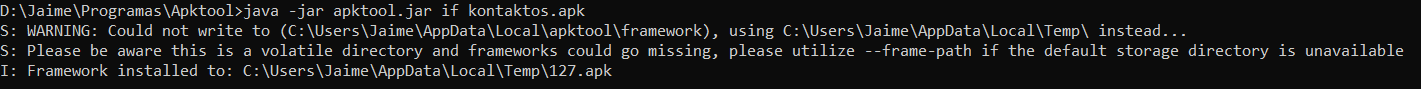
\includegraphics[width=\textwidth]{Punto41}
\caption{Ejecución de apktool para kontaktos.apk}
\label{Punto41}
\end{figure}

\item Se procede a decompilar la aplicación para su estudio. Véase la figura \ref{Punto42}.

\begin{figure}[h]
\centering
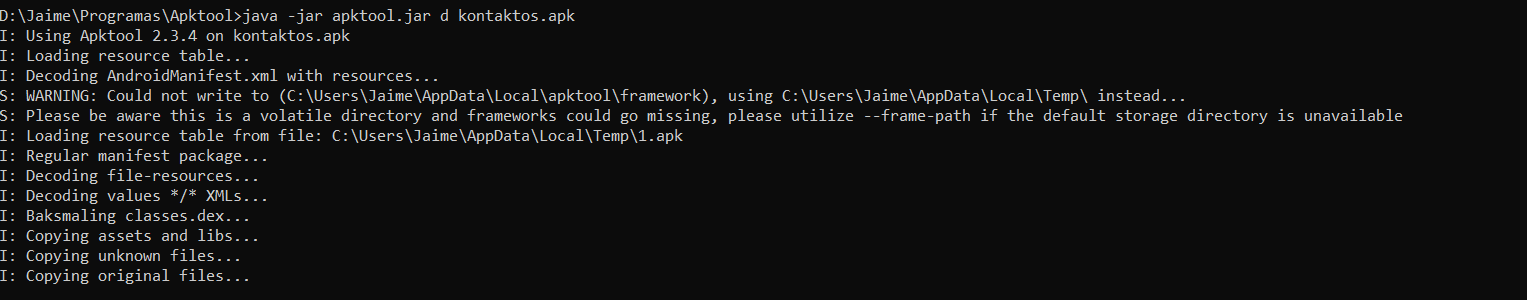
\includegraphics[width=\textwidth]{Punto42}
\caption{Decompilación de kontaktos.apk}
\label{Punto42}
\end{figure}

\item Se generará automáticamente un directorio que contiene la aplicación decompilada. Véase la figura \ref{Punto43}.

\begin{figure}[h]
\centering
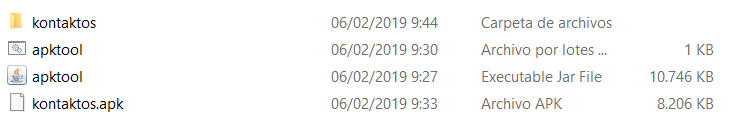
\includegraphics[width=\textwidth]{Punto43}
\caption{Aplicación decompilada}
\label{Punto43}
\end{figure}

\item Abrimos el fichero \emph{AndroidManifest.xml} para comprobar los permisos. Véase la figura \ref{Punto44}.

\begin{figure}[h]
\centering
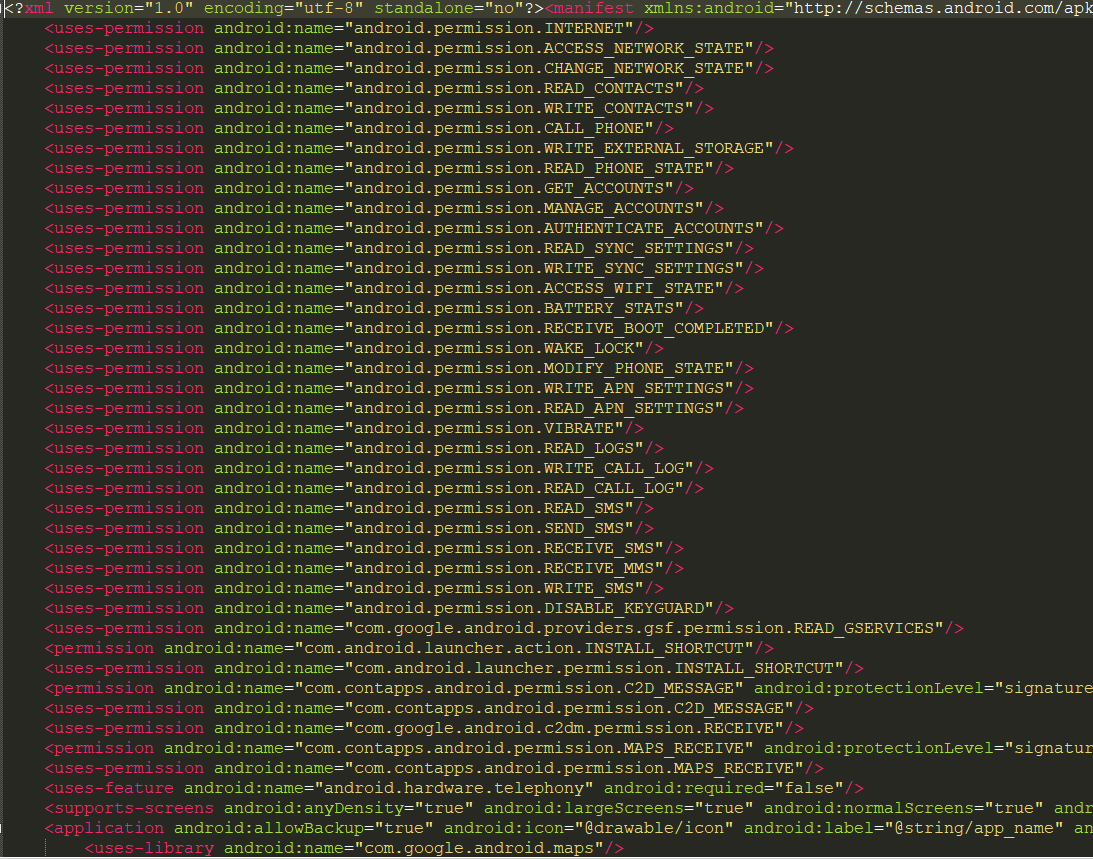
\includegraphics[width=\textwidth]{Punto44}
\caption{AndroidManifest.xml de la aplicación}
\label{Punto44}
\end{figure}

\end{enumerate}

Como se puede observar, esta aplicación requiere numerosos permisos, algunos de ellos son:

\begin{description}
\item[READ\_{}CONTACTS.] Permite a la aplicación la lectura de contactos del dispositivo.
\item[VIBRATE.] Permite a la aplicación vibrar.
\item[INTERNET.] Permite a la aplicación abrir sockets de red.
\item[CALL\_{}PHONE.] Permite a la aplicación efectuar una llamada telefónica sin hacer uso del teclado.
\item[BATTERY\_{}STATS.] Permite a la aplicación conocer las estadísticas de la batería del dispositivo.
\end{description}

Los \emph{permisos runtime} solo están disponibles a partir de Android 6.0 (API 23), son notificados al usuario cuando se ejecuta la aplicación, no en el momento de instalación. Estos permisos se pueden aceptar o denegar, para que no se pregunte al usuario cada vez que inicia la aplicación. Sin embargo, los \emph{permisos estáticos} son aquellos que están disponibles en versiones anteriores a 5.1 (API 22) y son notificados al usuario en el momento de instalación de la aplicación.

\clearpage
\section{Firmas y certificados}

En esta sección, se procederá a estudiar las firmas y los certificados digitales de la aplicación anterior. 

Lo primero que se debe hacer es instalar la aplicación en nuestro dispositivo virtual (AVD), para ello, se inicializa nuestro dispositivo virtual y una terminal para instalar el .apk, véase la figura .

\begin{figure}[h]
\centering
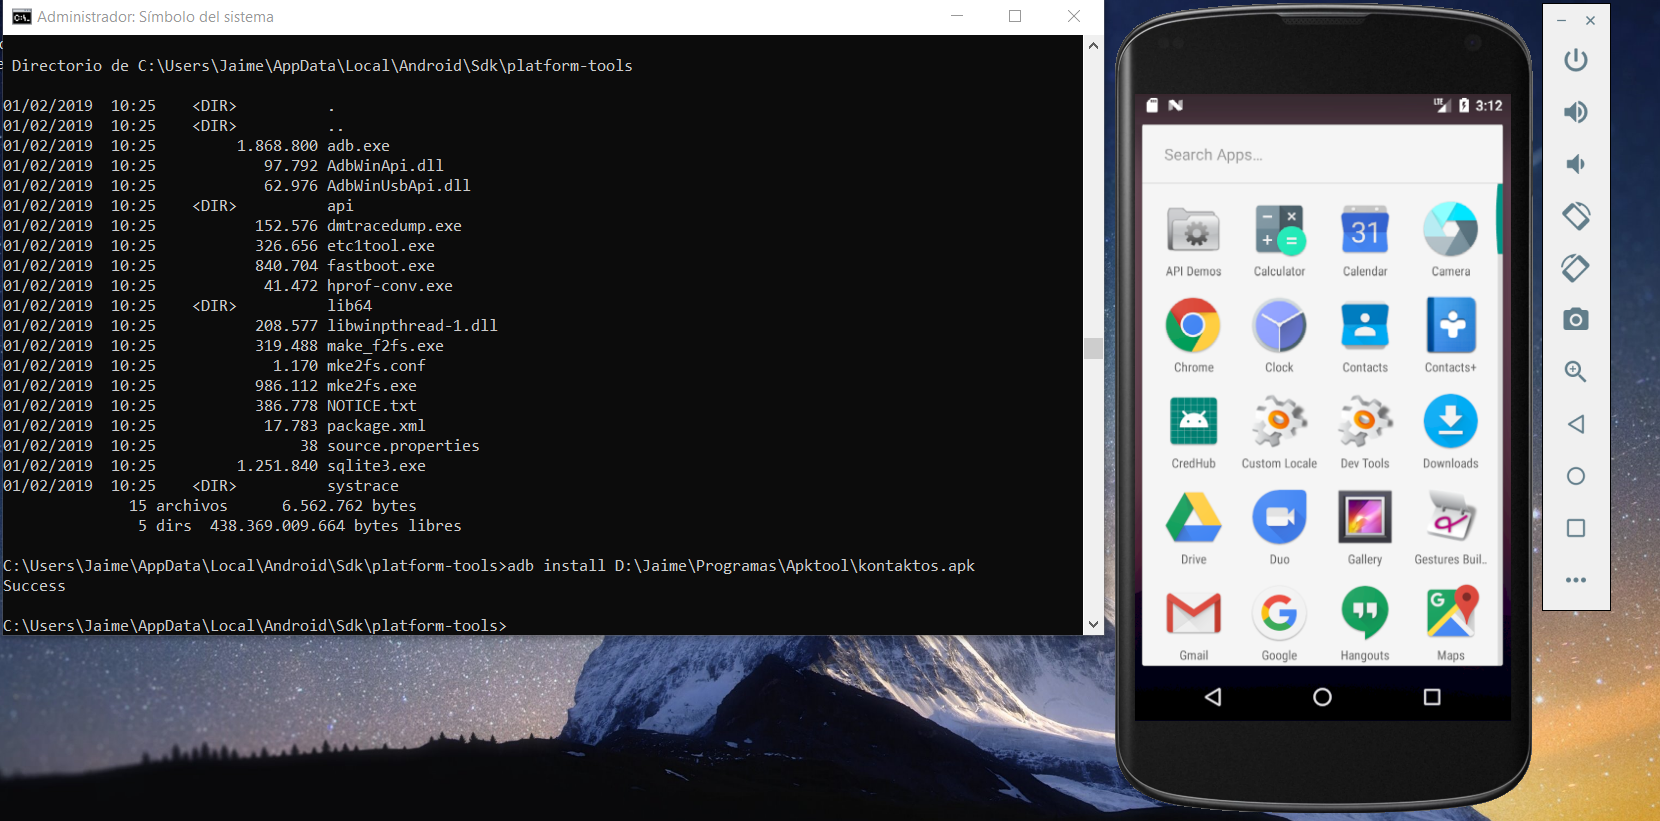
\includegraphics[width=\textwidth]{Punto51}
\caption{Instalación de una apk vía adb}
\label{Punto51}
\end{figure}

Seguidamente, se procede a descomprimir el .apk para visualizar los certificados, que se encuentran en el directorio "META-INF". Se descomprime la aplicación haciendo uso de la herramienta \emph{Winrar}. A continuación, hacemos uso de la herramienta \emph{keytool} para visualizar el contenido del certificado digital declarado por el dueño de la llave pública, véase la figura \ref{Punto52}.

\begin{figure}[h]
\centering
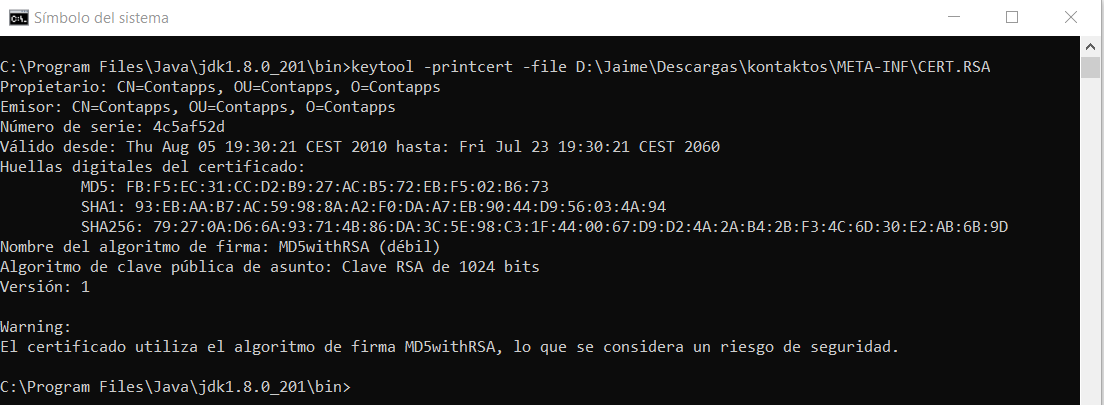
\includegraphics[width=\textwidth]{Punto52}
\caption{Certificado de la apk}
\label{Punto52}
\end{figure}
\clearpage

Como se puede comprobar, el certificado consta de varias partes, son las siguientes:

\begin{description}
\item[Propietario.] Propietario de la aplicación.
\item[Emisor.] Emisor de la aplicación.
\item[\#{} Serie.] Número de serie de la aplicación.
\item[Validez.] Indica el periodo de validez del certificado.
\item[Huellas digitales.] Funciones resumen únicas que identifican la aplicación.
\item[Algoritmo de firma.] Algoritmo de firmado utilizado en la aplicación.
\item[Algoritmo de clave pública.] Algoritmo utilizado para generar la clave pública.
\item[Versión.] Versión de la aplicación.
\end{description}

Los valores obtenidos de la aplicación \emph{kontaktos}, son los siguientes:


\begin{table}[h]
		\centering
		\begin{tabular}{|l|l|}
		\hline Serial number & 4c5af52d \\
		\hline Validez & Aug 2010 - Jul 2060 \\
		\hline Codificación clave pública & RSA \\
		\hline Tamaño clave pública & 1024 bits \\
		\hline Modulus & ?????????\\
		\hline Algoritmo firma & MD5withRSA \\
		\hline
		\end{tabular}	
\end{table}


La siguiente tarea consiste en obtener los hash criptográficos del logotipo de la aplicación y de al menos tres imágenes distintas que tengan densidad de pixeles diferentes, por ello, se debe analizar el fichero CERT.SF que se puede visualizar con cualquier editor de texto, en este caso, \emph{Notepad ++}. 

El fichero contiene más de 5000 líneas de código, así que, para localizar el nombre del icono de la aplicación se accede al directorio "res" y se busca el icono en los diferentes subdirectorios. El logo de la aplicación recibe el nombre de \emph{icon}, así que, se busca en el fichero este archivo y se encuentra su información:

\begin{quote}
\centering
Name: res/drawable-hdpi/icon.png

SHA1-Digest: X5/mtN+YdCFiZSlqEC9QRQ4eXFo=
\end{quote}

Para localizar tres imágenes diferentes se realiza de manera análoga, siendo cada directorio la densidad de pixeles de cada una, por ejemplo, mdpi (medium-dpi), hdpi (large-dpi) \ldots Por tanto, tres archivos válidos serían:

\begin{quote}
\centering
Name: res/drawable-hdpi/welcome\_{}pic.png

SHA1-Digest: kEtv1qXDVEaipT5tpE6yJFbTVag=
\end{quote}

\begin{quote}
\centering
Name: res/drawable-ldpi/wizard\_{}thank\_{}you.png

SHA1-Digest: oaQL3lC7JfkqM+rjezbyhW9iO3A=
\end{quote}


\begin{quote}
\centering
Name: res/drawable-mdpi/wizard\_{}free\_{}sms\_{}pic.png

SHA1-Digest: aiczu6u6zKX4kkjBzKZmODovr44=
\end{quote}


Para la codificación del hash, se ha utilizado el algoritmo \emph{SHA-1}, que separa la información en bloques de 512 bits y luego añade 80 vueltas utilizando una serie de vectores y mezclando la información con los siguientes hasta obtener un resumen de 160 bits.


\end{document}